\documentclass[12pt,compress,ngerman,utf8,t]{beamer}
\usepackage[ngerman]{babel}
\usepackage{calc}
\usepackage{ragged2e,wasysym,multicol}
\usepackage[protrusion=true,expansion=true]{microtype}

\hypersetup{colorlinks=true}

\title[Superturingmaschinen]{Superturingmaschinen}
\author[Ingo Blechschmidt]{\textcolor{white}{Ingo Blechschmidt}}
\date[2016-10-04]{\vspace*{-4em}\ \\\textcolor{white}{\scriptsize Augsburger Curry-Club \\ 4.
Oktober 2016}}

\usetheme{Warsaw}

\useinnertheme{rectangles}

\usecolortheme{seahorse}
\definecolor{mypurple}{RGB}{150,0,255}
\setbeamercolor{structure}{fg=mypurple}
\definecolor{myred}{RGB}{150,0,0}
\setbeamercolor*{title}{bg=myred,fg=white}
\setbeamercolor*{titlelike}{bg=myred,fg=white}

\usefonttheme{serif}
\usepackage[T1]{fontenc}
\usepackage{libertine}

\newcommand{\NN}{\mathbb{N}}

\newcommand{\slogan}[1]{%
  \begin{center}%
    \setlength{\fboxrule}{2pt}%
    \setlength{\fboxsep}{8pt}%
    {\usebeamercolor[fg]{item}\fbox{\usebeamercolor[fg]{normal text}\parbox{0.91\textwidth}{#1}}}%
  \end{center}%
}

\setbeamertemplate{navigation symbols}{}
\setbeamertemplate{headline}{}

\setbeamertemplate{title page}[default][colsep=-1bp,rounded=false,shadow=false]
\setbeamertemplate{frametitle}[default][colsep=-2bp,rounded=false,shadow=false,center]

\newcommand*\oldmacro{}%
\let\oldmacro\insertshorttitle%
\renewcommand*\insertshorttitle{%
  \oldmacro\hfill\insertframenumber\,/\,\inserttotalframenumber\hfill}

\newcommand{\hil}[1]{{\usebeamercolor[fg]{item}{\textbf{#1}}}}
\setbeamertemplate{frametitle}{%
  \vskip1em%
  \leavevmode%
  \begin{beamercolorbox}[dp=1ex,center]{}%
      \usebeamercolor[fg]{item}{\textbf{\textsf{\Large \insertframetitle}}}
  \end{beamercolorbox}%
}

\setbeamertemplate{footline}{%
  \leavevmode%
  \hfill%
  \begin{beamercolorbox}[ht=2.25ex,dp=1ex,right]{}%
    \usebeamerfont{date in head/foot}
    \insertframenumber\,/\,\inserttotalframenumber\hspace*{1ex}
  \end{beamercolorbox}%
  \vskip0pt%
}

\newcommand{\backupstart}{
  \newcounter{framenumberpreappendix}
  \setcounter{framenumberpreappendix}{\value{framenumber}}
}
\newcommand{\backupend}{
  \addtocounter{framenumberpreappendix}{-\value{framenumber}}
  \addtocounter{framenumber}{\value{framenumberpreappendix}}
}

\setbeameroption{show notes}
\setbeamertemplate{note page}[plain]

\begin{document}

% http://www.ufointernationalproject.com/wp-content/uploads/2015/11/a23.jpg
{\usebackgroundtemplate{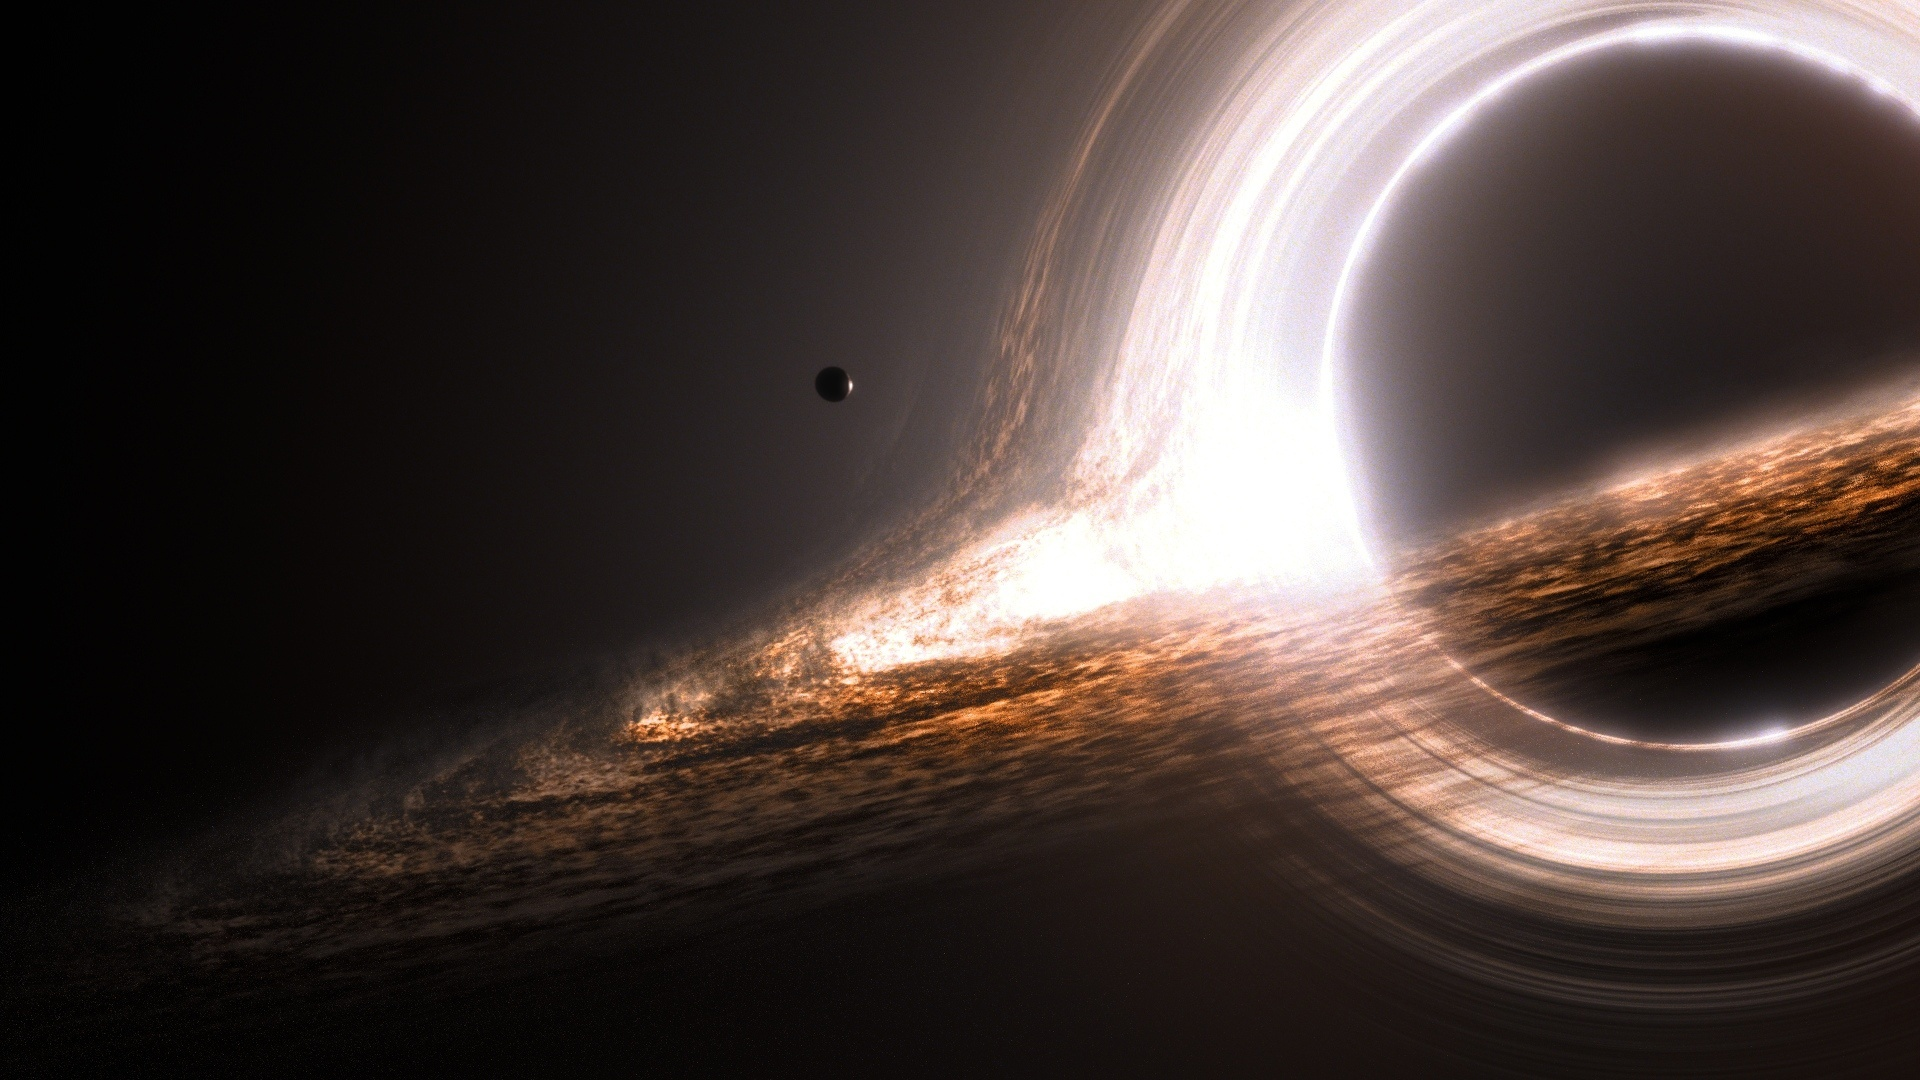
\includegraphics[height=\paperheight]{images/interstellar}}
\frame{\vspace*{12em}\titlepage}
\frame{\tableofcontents}}

\section{Erinnerungen}

\subsection{Gewöhnliche Turingmaschinen}
\begin{frame}{Ein Hoch auf Turingmaschinen}
  \begin{center}
    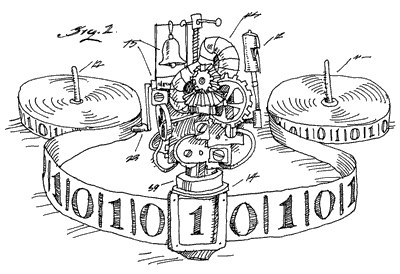
\includegraphics[width=0.6\textwidth]{images/turing-machine}
  \end{center}

  \begin{multicols}{2}
    \begin{enumerate}
      \item Schlichtheit
      \item Mechanischer Bezug
      \item Robustheit des Konzepts
      \item Äquivalenz zu anderen Modellen
      \item Querverbindungen
    \end{enumerate}
  \end{multicols}
\end{frame}
% mündlich: Es gibt Turingmaschinen mit 2 Zuständen und 4 Symbolen
% sowie mit 3 Zuständen und 3 Symbolen, deren Halteverhalten unbekannt ist.

\begin{frame}{Fun Facts zu Turingmaschinen}
  \begin{enumerate}
    \item Schon kleine Turingmaschinen sind diffizil.
    \item Es gibt Turingmaschinen, deren Halteverhalten unabhängig von
    Standard-Axiomen der Mathematik ist.
    % Zum Beispiel: die TM, die nach einem Widerspruch in ZFC sucht.
    % Wenn ZFC konsistent ist, dann hält diese nicht.
    % Dieser Umstand ist aber nicht in ZFC beweisbar (Gödel II).
    \pause

    \item Alle sinnvollen Modelle für Berechenbarkeit stimmen für
    Funktionen~$\NN \to \NN$ überein.
    % Aber nicht für Funktionen höherer Ordnung!
    \pause

    \item Eine Menge ist genau dann rekursiv aufzählbar, wenn
    sie durch eine~$\Sigma_1$-Aussage definierbar ist:
    \[ \{ n \in \NN \,|\, \text{es gibt $m \in \NN$ mit $\heartsuit$} \}, \]
    \pause
    und wenn sie diophantisch ist:
    \[ \{ n \in \NN \,|\, \text{die Gl. $f(n,x_1,\ldots,x_m) = 0$
    besitzt eine Lösung} \}, \]
    wobei $f$ ein Polynom mit ganzzahligen Koeffizienten ist.
  \end{enumerate}
\end{frame}


\subsection{Ordinalzahlen}

\begin{frame}{Ordinalzahlen messen Anordnung}
\end{frame}


\section{Grundlagen zu Superturingmaschinen}

\subsection{Erste Schritte}

\begin{frame}{Was sind Superturingmaschinen?}
  Bei Superturingmaschinen ist die Zeitachse spannender:
  \begin{itemize}
    \item normal: $0,\ 1,\ 2,\ \ldots$
    \item super:\phantom{rl} $0,\ 1,\ 2,\ \ldots,\ \omega,\ \omega + 1,\ \ldots,\ 2\omega,\ 2\omega
    + 1,\ \makebox[\widthof{R}][l]{$\ldots\ldots\ldots\ldots\ldots\ldots$}$
  \end{itemize}
  \bigskip

  Wird eine Limesordinalzahl erreicht, so wird
  \begin{itemize}
    \item die Maschine in einen designierten Zustand versetzt und
    \item der "`lim sup"' der vorherigen Bandinhalte genommen.
  \end{itemize}

  \begin{center}
    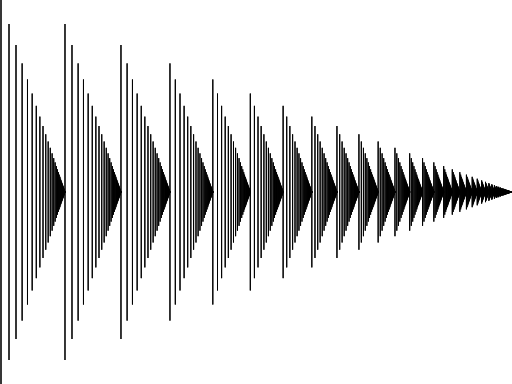
\includegraphics[width=0.35\textwidth]{images/ordinal-omega-squared}
  \end{center}
\end{frame}

\begin{frame}{Was können Superturingmaschinen?}
  \begin{itemize}
    \item Alles, was gewöhnliche Turingmaschinen können.
    \item Zahlentheoretische Behauptungen überprüfen:
      \begin{itemize}
        \item $\forall$ -- "`Für alle Zahlen gilt \ldots"'    % omega
        \item $\exists$ -- "`Es gibt eine Zahl mit \ldots"'   % omega
        \item $\forall\,\exists$ -- "`Für alle Zahlen~$n$
        gibt es jeweils eine Zahl~$m$ mit \ldots"'            % 2 omega
        \item $\exists\,\forall$ -- "`Es gibt eine Zahl~$n$,
        sodass für alle Zahlen~$m$ gilt: \ldots"'             % omega
        \item $\forall\,\exists\,\forall$                     % omega^2
        \item $\exists\,\forall\,\exists$
      \end{itemize}
    \item Entscheiden, ob gewöhnliche Turingmaschinen halten.
    \item Superturingmaschinen und verwandte Maschinen emulieren.
  \end{itemize}
  \pause

  \hil{Aber:} Superturingmaschinen können nicht alle Funktionen $\NN \to \NN$ berechnen.
  % Es gibt~$2^{\aleph_0}$ viele Funktionen $\NN \to \NN$, aber nur $\aleph_0$
  % viele Superturingmaschinen.
\end{frame}


\section{Besondere Phänomene}

\subsection{Stempelbare Ordinalzahlen}

\begin{frame}{Stempelbare Ordinalzahlen}
  Eine Ordinalzahl~$\alpha$ ist genau dann \hil{stempelbar} (clockable),
  falls es eine Superturingmaschine gibt, die genau nach Schritt~$\alpha$ hält.

  \begin{enumerate}
    \item Jede endliche Ordinalzahl ist stempelbar.
    \item Stempelbar sind außerdem: $\omega$, $2\omega$, $\omega^2$
    \item Sind~$\alpha$ und~$\beta$ stempelbar, so auch~$\alpha+\beta$
    und~$\alpha \cdot \beta$.
    \item Nur abzählbar viele Ordinalzahlen sind stempelbar.
    \pause
    \item Jede rekursive Ordinalzahl ist stempelbar.
    \item Beschleunigungssatz: Ist~$\alpha + n$ stempelbar, so auch~$\alpha$.
    \pause
    \item Große-Lücken-Satz: Für jede stempelbare Ordinalzahl~$\alpha$
    gibt eine Lücke der Länge~$\geq \alpha$ in den stempelbaren Ordinalzahlen.
    \item Viele-Lücken-Satz: Ist~$\alpha$ eine schreibbare Ordinalzahl,
    so gibt es mindestens~$\alpha$ viele Lücken der Länge~$\geq \alpha$ in den
    stempelbaren Ordinalzahlen.
    % Lückenlose-Blöcke-Satz?
  \end{enumerate}
\end{frame}

\end{document}

Ein Hoch auf Turingmaschinen
* Einfachheit
* Maschinelle Umsetzung klar
* Robustheit des Konzepts
* Äquivalenz zu anderen Modellen (aber nur für N --> N)
* Verbindungen zur Logik
* (aber: "TM sind nicht alles", siehe zum Beispiel R-Maschinen oder QTM)

Crashkurs Ordinalzahlen

Erste Schritte mit Superturingmaschinen
* Definition
* Beispielaufgaben
* Halteproblem
* Schwerere Aufgaben

Besondere Phänomene
* Ausbrechen aus Wiederholungen
* Lost Melody
* Abmessbare Ordinalzahlen

Effektiver Topos

"Allgemein sollten im Vortrag auch Maschinen vorgeführt werden, deren
Halteverhalten von mengentheoretischen Eigenschaften abhängt. Zum Beispiel die
Sache mit der Unabhängigkeit von BB(n) für kleine Wert von n von Adam Yedidia
und Scott Aaronson. http://www.scottaaronson.com/busybeaver.pdf"
